\section{Week 3-4}
\subsection{Objective}
This week, we will study and implement the variational inference framework with the objective of
estimating the posterior in a way that is indifferent to the type of regression performed.
We are going to pose the problem as an optimization problem and then derive an objective function that we can optimize over.
We will then try to implement it and perform some adjustments for efficiency and numerical stability.
% The objective of this week is to learn about and implement variational inference for Bayesian linear regression. 
% Then we will study convergence rates and accuracy by playing around with different parameters.
\subsection{Theory}
\subsubsection{Variational Inference and Variational Families}
In week 1, we were able to calculate the exact posterior using the right assumption and conjugacy between the prior and likelihood.
This turns out to be a rarity - in most cases, a closed form solution for the posterior is not readily available.
A common approach to this problem is to approximate the posterior distribution, using a \textit{variational distribution} $q$ picked from a family of distributions 
that we might imagine could approximate the posterior.
By picking a suitable objective function, we can use optimization techniques to pick a suitable $q$.
This is called \textit{variational inference}. Thus, our goal is to find a $q$ such that for any $\theta\in \Theta$, $q(\theta) \approx p(\theta | \B{y}, \B{d})$.
\subsubsection{Deriving a Suitable Objective Function}
Without any further assumptions about our variational distribution, an immediate idea could be to use the KL-divergence between $q$ and $p$ as an objective function:
\begin{equation}\label{eq:kld}q^*(\theta) = \arg \min_{q} \textsc{KL}(q(\theta) || p(\theta | \B{y}, \B{d}))\end{equation}
Calculating this requires us to calculate the posterior, which we would like to avoid since we are often not guaranteed to be able to compute the evidence term $\log(p(\B{y} | \B{d}))$ from \eqref{eq:bayes-rule}.
We can however rewrite the KL-divergence as follows \cite{blei17}:
\begin{equation}\textsc{KL}(q(\theta)|| p(\theta| \B{y}, \B{d})) = \mathbb{E}_{\theta \sim q}[\log q(\theta)] - \mathbb{E}_{\theta \sim q}[\log p(\theta|\B{y}, \B{d})]\end{equation}
and by conditioning
\begin{equation}\label{eq:kld-2}= \mathbb{E}_{\theta \sim q}[\log q(\theta)] - \mathbb{E}_{\theta \sim q}[\log p(\theta, \B{y}| \B{d})] - \log p(\B{y}| \B{d})\end{equation}
One can now notice that the last term is actually constant with regards to $q$.
Thus, when we optimize, we can ignore it. The remaining terms form the negative \textit{evidence lower bound} (ELBO) \cite{blei17}:
\begin{equation}\label{eq:elbo-1}\textsc{ELBO}(q)= -\textsc{KL}(q(\theta) || p(\theta | \B{y}, \B{d})) + \textrm{const}= \mathbb{E}_{\theta \sim q}[\log p(\theta, \B{y}| \B{d})]-\mathbb{E}_{\theta \sim q}[\log q(\theta)]\end{equation}
Since the KL-divergence consists of the negative ELBO and a constant, we can minimize the KL-divergence by maximizing the ELBO. Thus, we can reformulate our objective:
\begin{equation}\label{eq:elbo-objective}q^*(\theta) = \arg \max_{q} \textsc{ELBO}(q)\end{equation}
We can derive \eqref{eq:elbo-1} to a more easily computable term:
\begin{equation}\label{eq:elbo-2}\textsc{ELBO}(q) = \mathbb{E}_{\theta \sim q}[\log (p(\B{y}| \theta , \B{d})p(\theta | \B{d}))] - \mathbb{E}_{\theta \sim q}[\log q(\theta)]\end{equation}
\begin{equation}= \mathbb{E}_{\theta \sim q}[\log p(\B{y}| \theta , \B{d})]+\mathbb{E}_{\theta \sim q}[\log p(\theta | \B{d})] - \mathbb{E}_{\theta \sim q}[\log q(\theta)]\end{equation}
Using that $\theta$ is independent of $\B{d}$, we have
\begin{equation}= \mathbb{E}_{\theta \sim q}[\log p(\B{y}| \theta , \B{d})]-(-\mathbb{E}_{\theta \sim q}[\log p(\theta)] + \mathbb{E}_{\theta \sim q}[\log q(\theta)])\end{equation}
\begin{equation}= \mathbb{E}_{\theta \sim q}[\log p(\B{y}| \theta , \B{d})]-\mathbb{E}_{\theta \sim q}\left[\log \left(\frac{q(\theta)}{p(\theta)}\right)\right]\end{equation}
Using the definition of the KL-divergence:
\begin{equation}\label{eq:elbo-3}= \mathbb{E}_{\theta \sim q}[\log p(\B{y}| \theta , \B{d})]- \textsc{KL}(q || p)\end{equation}
Thus, this variational inference problem can work for any posterior, as long as one can calculate the expectation of the likelihood, and the KL-divergence between the variational distribution and the prior.
\subsubsection{The Linear Regression Case}
Let us now look at how one can find a good variational family for the linear regression case.
An easy guess would be to pick $q$ from a family of multivariate Gaussian distributions, since we know from conjugacy between the prior and likelihood that the posterior must also be multivariate Gaussian.
Thus, one can expect $q^*$ to be able to estimate $p$ perfectly.\\
This has the nice consequence of turning the KL-divergence into a closed form expression, since both $q$ and $p$ follow multivariate normal distributions \cite{kld-gaussian}.\\
\begin{equation}\textsc{KL}(q || p) = \frac{1}{2}\left(\textrm{tr} (\Sigma_p^{-1}\Sigma_q) + (\mu_p -\mu_q)^T\Sigma_p(\mu_p - \mu_q) - k + \log \frac{|\Sigma_p|}{|\Sigma_q|}\right)\end{equation}
We do have a problem, however: The first expectation of \eqref{eq:elbo-3} is an integral without a closed-form solution.
Thus, we wish to approximate it using Monte Carlo integration. 
To be able to sample $\theta$s from $q$, we will need to use the reparameterization trick:
By property of the multivariate normal distribution, there must exist some matrix $\B{A}$ such that $\theta \sim \mathcal{N}(\mu, \B{A} \B{A}^T)$ \cite{krause22}
and such that
\begin{equation}\theta = \mu + \B{A}\B{z}, \quad \textrm{where}\ \B{z}\sim \mathcal{N}(0,I_d)\end{equation}
Thus, we can simply sample N samples of $\B{z}$ and calculate $\theta$ from that. 
This means that our ELBO estimate can be written as follows:
\begin{equation}\textsc{ELBO}(q) \approx \frac{1}{N}\sum_{i=0}^N [\log p(\B{y} | \mu + \B{A}\B{z}^{(i)}, \B{d})] - \textsc{KL}(q || p)\label{eq:final-elbo}\end{equation}
$\mu$ and $\B{A}$ are then the parameters of $q$ that we will try to find through optimization.
% \subsubsection{Appendum: Using the ELBO as a proxy for the KL-divergence}
% When going from equation \ref{eq:kld-2} to \ref{eq:elbo-1}, we saw how the $\textsc{ELBO}$ is defined as the negative KLD plus the log-evidence $\log p(\B{y}|\B{d})$.
% The difference between the ELBO and the KLD is exactly this: the log-evidence.
\subsection{Implementation}
\subsubsection{Main Implementation}
The main work of the algorithm is in calculating the ELBO. This can then be plugged into the same optimizer as in week 2.
The ELBO can be implemented as follows in Python:
\begin{minted}{python}
def ELBO(d, y, mean, A): # optimizing for mean, A
  zs = np.random.normal(size=(N, len(mean))) # N samples of size d
  likelihood_samples = []
  for z in zs:
    theta = mean + A @ z
    likelihood_samples.append(log_likelihood(y, theta, d))
  return 1/N * np.sum(likelihood_samples, axis=0) - KLD(mean, A, prior_mean, prior_A)
\end{minted}
where the log-likelihood is implemented after \eqref{eq:likelihood}:
\begin{minted}{python}
def log_likelihood(y, theta, d):
  return log_pdf(y, theta @ d, noise * np.eye(len(theta)))
\end{minted}
and the KL-divergence like so
\begin{minted}{python}
def KLD(mean_q, A_q, mean_p, A_p):
    sigma_q = (A_q @ A_q.T)
    sigma_p = (A_p @ A_p.T)
    bar_sigma_q = np.linalg.det(sigma_q)
    bar_sigma_p = np.linalg.det(sigma_p)
    k = len(mean_q)
    return 0.5 * (np.trace(np.linalg.inv(sigma_p) @ sigma_q) + (mean_p - mean_q).T @ np.linalg.inv(sigma_p) @ (mean_p - mean_q) - k + np.log(bar_sigma_p/bar_sigma_q))
\end{minted}
\subsubsection{Optimizing over a Mean and a Matrix}
Like in week 2, it is not trivial to optimize over both a mean and a matrix. Thus, we will encode $\mu$ and $\B{A}$ as a vector $\B{v}$ of the shape
$$\B{v}=\begin{bmatrix}\mu_0 \\ \vdots \\ \mu_d \\ \B{A}_{1,1} \\ \vdots \\ \B{A}_{1,d} \\ \B{A}_{2,1} \\ \vdots \\ \B{A}_{d, d}\end{bmatrix}$$
whenever we need to take the gradient or regard them in the context of the optimizer.
The following help functions can help encode and decode $\mu$ and $\B{A}$:
\begin{minted}{python}
def encode_q_params(q_params): # mean, A to vector
    mean, A = q_params
    return np.array(list(mean) + list(A.flatten()))
def decode_q_params(encoded_q, dim = 3): # vector to mean, A
    shape = len(encoded_q)
    A_shape = (int(np.sqrt(shape - dim)), int(np.sqrt(shape - dim)))
    mean = encoded_q[0:dim]
    A = encoded_q[dim:shape].reshape(A_shape)
    return mean, A
\end{minted}
\subsection{Results}
\begin{figure}[H]
  \centering
  \begin{subfigure}{0.4\textwidth}
    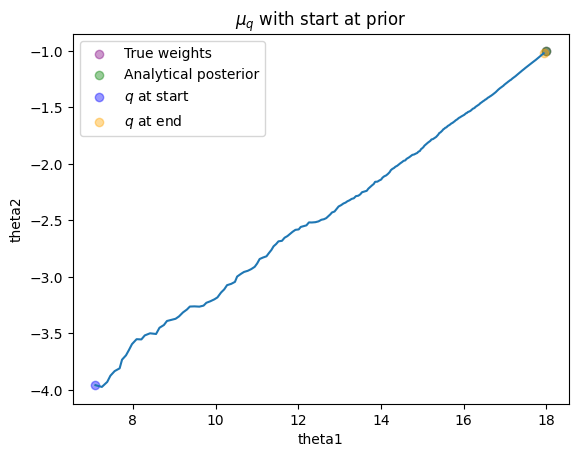
\includegraphics[width=\textwidth]{week3/mu-walk-1.png}
  \end{subfigure}
  \begin{subfigure}{0.4\textwidth}
    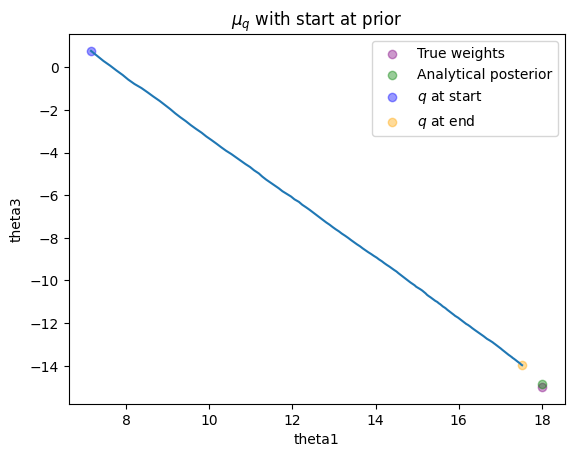
\includegraphics[width=\textwidth]{week3/mu-walk-2.png}
  \end{subfigure}
  \caption{Change in mean of $q$ after 200 iterations of the algorithm with $N$ = 10, $\ell = 100$.}
  \label{fig:mu-walk}
\end{figure}
\begin{figure}[H]
  \centering
  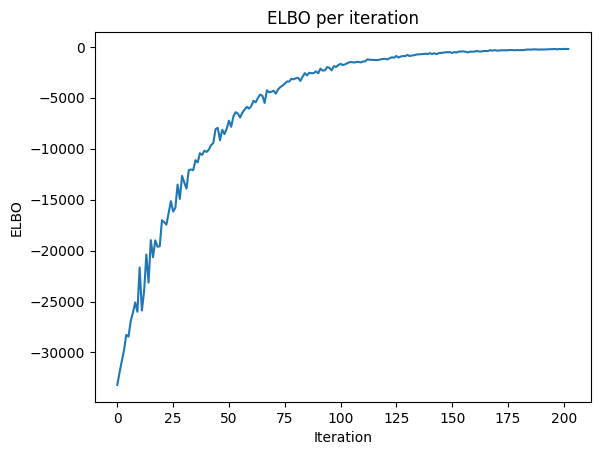
\includegraphics[width=0.5\textwidth]{week3/elbo-per-iter.png}
  \caption{ELBO after each iteration of the algorithm with $N$ = 10, $\ell = 100$.}
  \label{fig:elbo}
\end{figure}
As one can see in Figure \ref{fig:mu-walk}, the mean of $q$ confidently moves towards the analytical posterior (and true weights).
It can also been seen in Figure \ref{fig:elbo} that the ELBO converges after 200 or so iterations, indicating that we have indeed found an optimum.
\subsection{Evaluation}
The algorithm presented here works as expected, and functions as a possible replacement for the analytical posterior.
We've been able to utilize the ELBO as a proxy for the KL-divergence and created a framework that can fitted to many different kind of regression problems, 
as long as one can estimate the log-likelihood and compute the KL-divergence between the variational distribution and the prior.

